% !TeX program = xelatex
\documentclass{nwputhesis}
\usepackage{gbt7714}
\begin{document}

% 生成封面, 使用\maketitle 
% 该封面不同学院要求可能不同,如有需要,请在cls文件中自行修改
\maketitle

\newpage
% 目录
\makecontent
\iffalse
    \makefigcontent
    \maketabcontent
\fi
% 正文
\maketext

\section{实习目标}
\subsection{学习方向及目标}
学习现在先进的计算机视觉(Computer Vision)以及图形学与AI结合的模型如Neural Radiance Fields(神经辐射场,简称NeRF),3D Gaussian Splatting(3D高斯溅射,简称3dgs),以及YOLO(全称You Only Look Once),同时理解各个模型的实现原理。
\subsection{期望}
\begin{itemize}
    \item 完成搭建尽可能多的AI模型,配置其环境,并完成训练其预设数据库。
    \item 学习并理解各个模型的实现原理。
    \item 自己制作数据并通过基于AI的三维重建制作模型。
\end{itemize}
\makespace
\section{信号模型}
\subsection{公式}
\subsubsection{简单公式}
\begin{equation}
    \int_a^b f(x)\mathrm{d}x=F(b)-F(a)
\end{equation}

\subsubsection{多行公式}
如公式(\ref{q1})所示。
\begin{equation}
    \label{q1}
    \begin{aligned}
        dx      & =v_{x}dt  \\
        dy      & =v_{y}dt  \\
        x_{t+1} & =dx+x_{t} \\
        y_{t+1} & =dx+y_{t}
    \end{aligned}
\end{equation}

\subsubsection{括号公式}
如公式(\ref{q1})所示。
\begin{equation}
    \left\{
    \begin{aligned}
        100(t-kT_{2}) & , & t\in (kT_{2}, kT_{2}+0.2 )    \\
        20            & , & t\in (kT_{2}+0.2,kT_{2}+2.2)  \\
        -100t+240     & , & t\in( kT_{2}+2.2, kT_{2}+2.4) \\
        0             & , & t\in (kT_{2}+2.4,(k+1)T_{2})
    \end{aligned}
    \right.
\end{equation}

\subsection{表格}
\subsubsection{简单表格}
如表\ref{table1}所示。

\begin{table}[H]
    \fontsize{10.5bp}{1.25}
    \caption{表格标题}
    % \setlength{\abovecaptionskip}{0.2cm}  %调整标题与图距离
    % \setlength{\belowcaptionskip}{0.2cm} %调整标题与下文距离
    \centering\label{table1}
    % \vspace{-0.5em}	
    \begin{tabular}{|c|c|c|c|}
        \hline % \toprule[1.5pt]
        方法       & A算法 & B算法 & C算法 \\ \hline
        误差/dB    & 0.86  & 1.02  & 0.69  \\ \hline
        计算时间/s & 25    & 25    & 27    \\ \hline
    \end{tabular}
\end{table}

\subsubsection{三线表}
三线表参考表\ref{table3}
\begin{table}[H]
    \fontsize{10.5bp}{1.25}
    \caption{表格标题}
    % \setlength{\abovecaptionskip}{0.2cm}  %调整标题与图距离
    % \setlength{\belowcaptionskip}{0.2cm} %调整标题与下文距离
    \centering\label{table3}
    % \vspace{-0.5em}	
    \begin{tabular}{cccc}
        \toprule[1.5pt]
        方法       & A算法 & B算法 & C算法 \\
        \toprule[1.5pt]
        误差/dB    & 0.86  & 1.02  & 0.69  \\
        计算时间/s & 25    & 25    & 27    \\
        \toprule[1.5pt]
    \end{tabular}
\end{table}

\subsubsection{精排表格}
较为复杂的表格参考表\ref{table2}
\begin{table}[H]
    \caption{表格标题}
    % \setlength{\abovecaptionskip}{0.2cm}  %调整标题与图距离
    % \setlength{\belowcaptionskip}{-0.2cm} %调整标题与下文距离
    \fontsize{10.5bp}{1.25}
    \centering\label{table2}
    % \vspace{-0.5em}	
    \begin{tabular}{|c|c|c|c|}
        \hline % \toprule[1.5pt]
        \makecell*[c]{ Parameter Group     \\ Condition Selection } &\makecell*[c]{ Basic Ways \\of Hatching  } 	& \makecell*[c]{Calculated Average\\ Alapsed Time} & \makecell*[c]{Calculated Average\\ Alapsed Time}  \\
        \hline
        \makecell*[c]{ Parameter group (1) \\ \\Parameter group (2)\\} &\makecell*[c]{ Zigzag   Hatch\\Contour Hatch\\Zigzag   Hatch\\Contour Hatch}& \makecell*[c]{468.940\\374.923 \\885.792\\1947.77}   & \makecell*[c]{Zigzag 1.888 \\ Contour  5.195   }   \\
        \hline
        \makecell*[c]{ Parameter group (1) \\ \\ Parameter group (2)\\}  &\makecell*[c]{ Zigzag   Hatch\\Contour Hatch\\Zigzag   Hatch\\Contour Hatch}&\makecell*[c]{ 545.080\\356.847\\1068.275\\1692.098} & \makecell*[c]{Zigzag 1.960 \\ Contour 4.742  }  \\
        \hline
    \end{tabular}
    % \vspace{-1.5em}
\end{table}

\subsection{图片}
\subsubsection{单个图片}
单图如图\ref{P1}所示。
\begin{figure}[!ht]
    \centering
    %\vspace{-0.30cm} %设置与上面正文的距离`
    %\setlength{\abovecaptionskip}{0.0cm}   %调整图片标题与图距离`
    %\setlength{\belowcaptionskip}{0.0cm} %调整图片标题与下文距离
    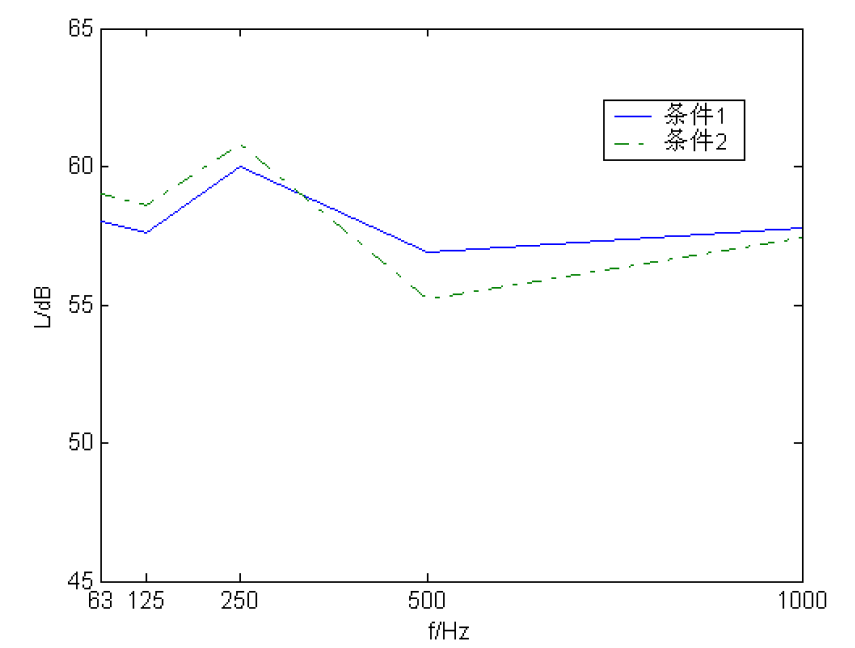
\includegraphics[width=4cm]{./picture/test.png}
    \caption{图片标题}\label{P1}
\end{figure}
\subsubsection{子图}
多子图如图\ref{P2}、\ref{P2.1}、\ref{P2.2}所示。
\begin{figure}[h!]
    \centering
    \begin{subfigure}[b]{0.25\linewidth}
        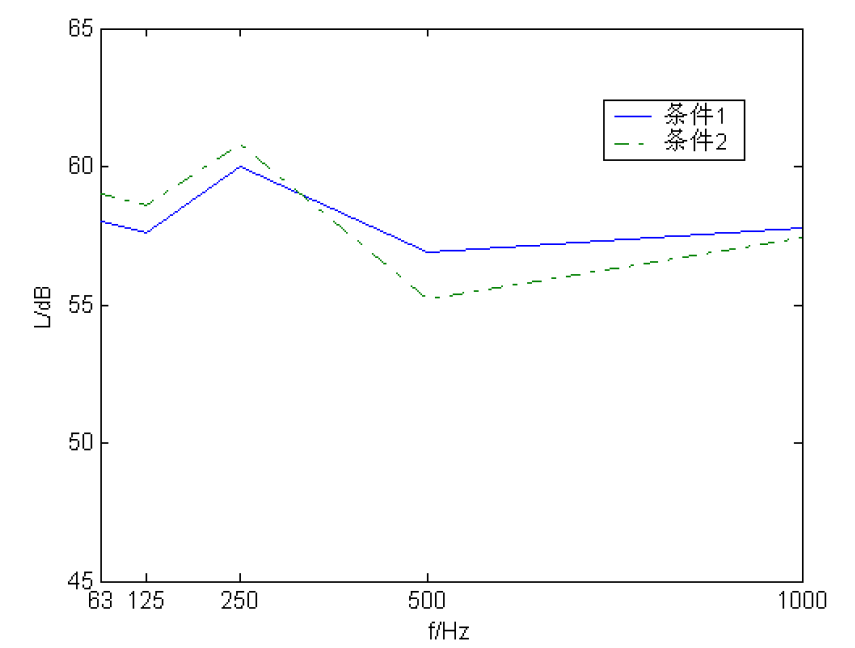
\includegraphics[width=\linewidth]{picture/test.png}
        \caption{图片标题1}\label{P2.1}
    \end{subfigure}
    \begin{subfigure}[b]{0.25\linewidth}
        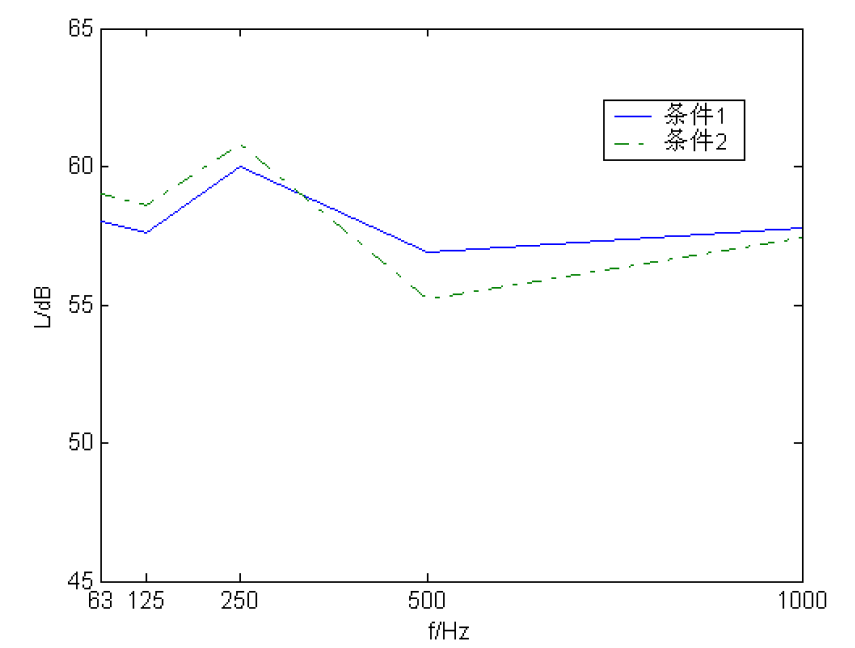
\includegraphics[width=\linewidth]{picture/test.png}
        \caption{图片标题2}\label{P2.2}
    \end{subfigure}
    \caption{总标题}
    \label{P2}
\end{figure}
\makespace
\section{英文标题Test}
\subsection{英文标题Test}
\subsubsection{英文标题Test}
% 参考文献
\makespace
\section*{参考文献}
\begingroup  % 去掉thebibliography环境自带的“参考文献”标题
\renewcommand{\section}[2]{}
\addcontentsline{toc}{section}{参考文献}
% npu专用
\bibliographystyle{gbt7714-numerical}
\addtolength{\itemsep}{-0.6em} % 缩小参考文献间的垂直间距
\begin{spacing}{1.0}           %段落行距设置
    \bibliography{reference/reference}
\end{spacing}
% 参考文献位置

% 致谢
\makespace %另起一页空两行
\section*{致谢}
\begin{center}
    { \blackti \fontsize{16.0600pt}{1.25}致 \, 谢}
\end{center}
\addcontentsline{toc}{section}{致\texorpdfstring{ \, }{} 谢}
\myspace{1}
致谢内容。

% 毕业设计小结
\section*{毕业设计小结}
\makespace
\begin{center}
    { \blackti \fontsize{16.0600pt}{1.25}毕业设计小结}
\end{center}
\addcontentsline{toc}{section}{毕业设计小结}
\myspace{1}
小结内容。

% 附录
\makespace
\section*{附录}
\begin{center}
    { \blackti \fontsize{16.0600pt}{1.25}附 \, 录}
\end{center}
\addcontentsline{toc}{section}{附\texorpdfstring{ \, }{} 录}
\myspace{1}
附录内容。
\end{document}

